\documentclass[12pt,a4paper]{report}
\usepackage[T2A]{fontenc}
\usepackage[utf8]{inputenc}
\usepackage[russian]{babel}
\usepackage{graphicx, setspace, amsmath, amsfonts}

\usepackage[
top = 1.25cm, 
bottom = 2.0cm]{geometry}

\begin{document}
\begin{titlepage} 
	\centering
    % HEADER
	{
        \scshape
        Федеральное государственное автономное образовательное учреждение высшего образования
        \par
        \textbf{«Научно-образовательная корпорация ИТМО»}
        \par
        \vspace*{1cm}
        Факультет Программной Инженерии и Компьютерной Техники
        \par
    }
    % LOGO
    \vspace*{0.6cm}
    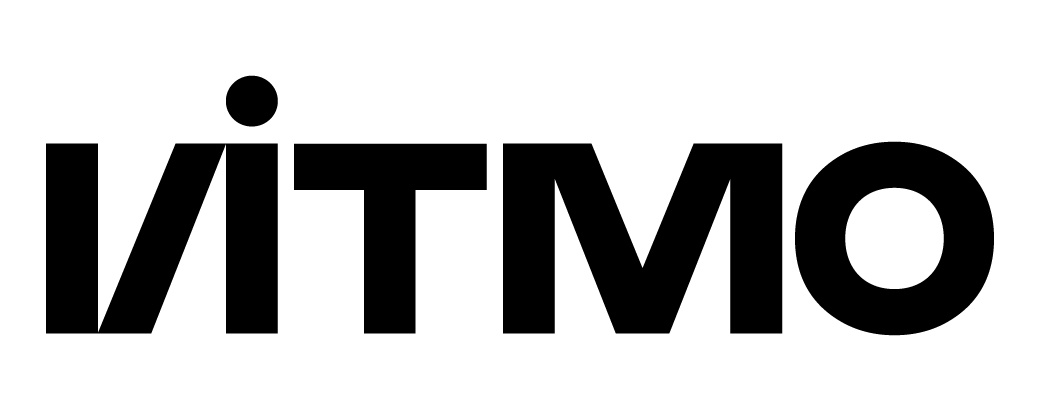
\includegraphics[width=\textwidth]{logo.png}
    % LAB INFO
    {
        \Large
        \textbf{Домашнее задание по теории графов №4}
        \par
        \normalsize
        \vspace*{0.75cm}
        \textbf{Вариант 92}
        \par
    }
    \vfill
    % СREDITS
    \hfill\begin{minipage}{\dimexpr\textwidth-7.8cm}
        \textbf{Выполнил:}\par
        Степанов Арсений Алексеевич\par
        \vspace*{0.15cm}
        \textbf{Группа:}\par
        P3109\par
        \vspace*{0.15cm}
        \textbf{Преподаватель:}\par
        Поляков Владимир Иванович\par
    \end{minipage}
    \vfill
    Санкт-Петербург, \the\year{}г.
\end{titlepage}  
\onehalfspacing
\section*{Матрица смежности графа}
\begin{tabular}{|c|c|c|c|c|c|c|c|c|c|c|c|c|c|}
    \hline
    V/V & $e_{1}$ & $e_{2}$ & $e_{3}$ & $e_{4}$ & $e_{5}$ & $e_{6}$ & $e_{7}$ & $e_{8}$ & $e_{9}$ & $e_{10}$ & $e_{11}$ & $e_{12}$ \\
    \hline
    $e_{1}$  &   &   &   & 5 &   &   &   & 4 & 1 & 4 &   & 1 \\
    \hline
    $e_{2}$  &   &   &   &   & 4 &   & 4 &   & 1 &   &   &   \\
    \hline
    $e_{3}$  &   &   &   & 5 &   & 4 & 3 & 4 &   & 3 & 3 &   \\
    \hline
    $e_{4}$  & 5 &   & 5 &   &   &   & 1 &   &   &   &   & 1 \\
    \hline
    $e_{5}$  &   & 4 &   &   &   & 4 & 4 &   &   &   &   & 5 \\
    \hline
    $e_{6}$  &   &   & 4 &   & 4 &   & 5 &   & 3 &   &   & 2 \\
    \hline
    $e_{7}$  &   & 4 & 3 & 1 & 4 & 5 &   & 2 &   &   & 5 &   \\
    \hline
    $e_{8}$  & 4 &   & 4 &   &   &   & 2 &   &   &   & 1 &   \\
    \hline
    $e_{9}$  & 1 & 1 &   &   &   & 3 &   &   &   & 4 & 4 &   \\
    \hline
    $e_{10}$ & 4 &   & 3 &   &   &   &   &   & 4 &   & 5 & 5 \\
    \hline
    $e_{11}$ &   &   & 3 &   &   &   & 5 & 1 & 4 & 5 &   & 2 \\
    \hline
    $e_{12}$ & 1 &   &   & 1 & 5 & 2 &   &   &   & 5 & 2 &   \\
    \hline
\end{tabular}

\section*{Найти гамильтонов цикл}
Включаем в S вершину $x_1. S = \{x_1\}$\\
Возможная вершина: $x_{4}. S = \{x_{1},x_{4}\}$\\
Возможная вершина: $x_{3}. S = \{x_{1},x_{4},x_{3}\}$\\
Возможная вершина: $x_{6}. S = \{x_{1},x_{4},x_{3},x_{6}\}$\\
Возможная вершина: $x_{5}. S = \{x_{1},x_{4},x_{3},x_{6},x_{5}\}$\\
Возможная вершина: $x_{2}. S = \{x_{1},x_{4},x_{3},x_{6},x_{5},x_{2}\}$\\
Возможная вершина: $x_{7}. S = \{x_{1},x_{4},x_{3},x_{6},x_{5},x_{2},x_{7}\}$\\
Возможная вершина: $x_{8}. S = \{x_{1},x_{4},x_{3},x_{6},x_{5},x_{2},x_{7},x_{8}\}$\\
Возможная вершина: $x_{11}. S = \{x_{1},x_{4},x_{3},x_{6},x_{5},x_{2},x_{7},x_{8},x_{11}\}$\\
Возможная вершина: $x_{9}. S = \{x_{1},x_{4},x_{3},x_{6},x_{5},x_{2},x_{7},x_{8},x_{11},x_{9}\}$\\
Возможная вершина: $x_{10}. S = \{x_{1},x_{4},x_{3},x_{6},x_{5},x_{2},x_{7},x_{8},x_{11},x_{9},x_{10}\}$\\
Возможная вершина: $x_{12}. S = \{x_{1},x_{4},x_{3},x_{6},x_{5},x_{2},x_{7},x_{8},x_{11},x_{9},x_{10},x_{12}\}$\\
Гамильтонов цикл найден. $S = \{x_{1},x_{4},x_{3},x_{6},x_{5},x_{2},x_{7},x_{8},x_{11},x_{9},x_{10},x_{12}\}$\\



\subsection*{Матрица смежности с перенумерованными вершинами}

\begin{tabular}{|c|c|c|c|c|c|c|c|c|c|c|c|c|c|} 
    \hline
    V/V & $e_{1}$ & $e_{2}$ & $e_{3}$ & $e_{4}$ & $e_{5}$ & $e_{6}$ & $e_{7}$ & $e_{8}$ & $e_{9}$ & $e_{10}$ & $e_{11}$ & $e_{12}$ \\
    \hline  
    $e_x$ &   &	1 &	0 &	0 &	0 &	0 &	0 &	1 &	0 &	1 &	1 &	1 \\
    \hline
    $e_x$ & 1 &	0 &	1 &	0 &	0 &	0 &	1 &	0 &	0 &	0 &	0 &	1 \\
    \hline
    $e_x$ &   &	1 &	0 &	1 &	0 &	0 &	1 &	1 &	1 &	0 &	1 &	0 \\
    \hline
    $e_x$ &   &	0 &	1 &	0 &	1 &	0 &	1 &	0 &	0 &	1 &	0 &	1 \\
    \hline
    $e_x$ &   &	0 &	0 &	1 &	0 &	1 &	1 &	0 &	0 &	0 &	0 &	1 \\
    \hline
    $e_x$ &   &	0 &	0 &	0 &	1 &	0 &	1 &	0 &	0 &	1 &	0 &	0 \\
    \hline
    $e_x$ &   &	1 &	1 &	1 &	1 &	1 &	0 &	1 &	1 &	0 &	0 &	0 \\
    \hline
    $e_x$ & 1 &	0 &	1 &	0 &	0 &	0 &	1 &	0 &	1 &	0 &	0 &	0 \\
    \hline
    $e_x$ &   &	0 &	1 &	0 &	0 &	0 &	1 &	1 &	0 &	1 &	1 &	1 \\
    \hline
    $e_x$ & 1 &	0 &	0 &	1 &	0 &	1 &	0 &	0 &	1 &	0 &	1 &	0 \\
    \hline
    $e_x$ & 1 &	0 &	1 &	0 &	0 &	0 &	0 &	0 &	1 &	1 &	0 &	1 \\
    \hline
    $e_x$ & 1 &	1 &	0 &	1 &	1 &	0 &	0 &	0 &	1 &	0 &	1 &	0 \\
    \hline
\end{tabular}\\
\hfill\break
До перенумерации: $\{x_{1}, x_{4}, x_{3}, x_{6}, x_{5}, x_{2}, x_{7}, x_{8}, x_{11}, x_{9}, x_{10}, x_{12}\}$\\
После перенумерации: $\{x_{1}, x_{2}, x_{3}, x_{4}, x_{5}, x_{6}, x_{7}, x_{8}, x_{9}, x_{10}, x_{11}, x_{12}\}$
\subsection*{Построение графа пересечений $G'$}
Определим $p_{212}$, для чего в матрице R выделим подматрицу $R_{212}$ \\
Ребро $(x_{2}x_{12})$ пересекается с $(x_{1}x_{8}),(x_{1}x_{10}),(x_{1}x_{11})$ \\
Определим $p_{311}$, для чего в матрице R выделим подматрицу $R_{311}$ \\
Ребро $(x_{3}x_{11})$ пересекается с $(x_{1}x_{8}),(x_{1}x_{10}),(x_{2}x_{7})$ \\
Определим $p_{39}$, для чего в матрице R выделим подматрицу $R_{39}$ \\
Ребро $(x_{3}x_{9})$ пересекается с $(x_{1}x_{8}),(x_{2}x_{7})$ \\
Определим $p_{38}$, для чего в матрице R выделим подматрицу $R_{38}$ \\
Ребро $(x_{3}x_{8})$ пересекается с $(x_{2}x_{7})$ \\
Определим $p_{412}$, для чего в матрице R выделим подматрицу $R_{412}$ \\
Ребро $(x_{4}x_{12})$ пересекается с $(x_{1}x_{8}),(x_{1}x_{10}),(x_{1}x_{11}),(x_{2}x_{7}),(x_{3}x_{7}),(x_{3}x_{8}),(x_{3}x_{9}),(x_{3}x_{11})$ \\
Определим $p_{410}$, для чего в матрице R выделим подматрицу $R_{410}$ \\
Ребро $(x_{4}x_{10})$ пересекается с $(x_{1}x_{8}),(x_{2}x_{7}),(x_{3}x_{7}),(x_{3}x_{8}),(x_{3}x_{9})$ \\
Определим $p_{512}$, для чего в матрице R выделим подматрицу $R_{512}$ \\
Ребро $(x_{5}x_{12})$ пересекается с $(x_{1}x_{8}),(x_{1}x_{10}),(x_{1}x_{11}),(x_{2}x_{7})$,\\
$(x_{3}x_{7}),(x_{3}x_{8}),(x_{3}x_{9}),(x_{3}x_{11}),(x_{4}x_{7}),(x_{4}x_{10})$ \\
Определим $p_{610}$, для чего в матрице R выделим подматрицу $R_{610}$ \\
Ребро $(x_{6}x_{10})$ пересекается с $(x_{1}x_{8}),(x_{2}x_{7}),(x_{3}x_{7}),(x_{3}x_{8}),(x_{3}x_{9}),(x_{4}x_{7}),(x_{5}x_{7})$ \\
\hfill\break
\footnotesize
\hspace*{-1cm}
\begin{tabular}{|c|c|c|c|c|c|c|c|c|c|c|c|c|c|c|c|c|}
    \hline
    & $p_{1 | 8}$ & $p_{2 | 12}$ & $p_{1 | 10}$ & $p_{1 | 11}$ & $p_{3 | 11}$ & $p_{2 | 7}$ & $p_{3 | 9}$ & $p_{3 | 8}$ & $p_{4 | 12}$ & $p_{3 | 7}$ & $p_{4 | 10}$ & $p_{5 | 12}$ & $p_{4 | 7}$ & $p_{6 | 10}$ & $p_{5 | 7}$ \\
    \hline
    $p_{1 | 8}$ & 1 & 1 & 0 & 0 & 1 & 0 & 1 & 0 & 1 & 0 & 1 & 1 & 0 & 1 & 0 \\
    \hline
    $p_{2 | 12}$ & 1 & 1 & 1 & 1 & 0 & 0 & 0 & 0 & 0 & 0 & 0 & 0 & 0 & 0 & 0 \\
    \hline
    $p_{1 | 10}$ & 0 & 1 & 1 & 0 & 1 & 0 & 0 & 0 & 1 & 0 & 0 & 1 & 0 & 0 & 0 \\
    \hline
    $p_{1 | 11}$ & 0 & 1 & 0 & 1 & 0 & 0 & 0 & 0 & 1 & 0 & 0 & 1 & 0 & 0 & 0 \\
    \hline
    $p_{3 | 11}$ & 1 & 0 & 1 & 0 & 1 & 1 & 0 & 0 & 1 & 0 & 0 & 1 & 0 & 0 & 0 \\
    \hline
    $p_{2 | 7}$ & 0 & 0 & 0 & 0 & 1 & 1 & 1 & 1 & 1 & 0 & 1 & 1 & 0 & 1 & 0 \\
    \hline
    $p_{3 | 9}$ & 1 & 0 & 0 & 0 & 0 & 1 & 1 & 0 & 1 & 0 & 1 & 1 & 0 & 1 & 0 \\
    \hline
    $p_{3 | 8}$ & 0 & 0 & 0 & 0 & 0 & 1 & 0 & 1 & 1 & 0 & 1 & 1 & 0 & 1 & 0 \\
    \hline
    $p_{4 | 12}$ & 1 & 0 & 1 & 1 & 1 & 1 & 1 & 1 & 1 & 1 & 0 & 0 & 0 & 0 & 0 \\
    \hline
    $p_{3 | 7}$ & 0 & 0 & 0 & 0 & 0 & 0 & 0 & 0 & 1 & 1 & 1 & 1 & 0 & 1 & 0 \\
    \hline
    $p_{4 | 10}$ & 1 & 0 & 0 & 0 & 0 & 1 & 1 & 1 & 0 & 1 & 1 & 1 & 0 & 0 & 0 \\
    \hline
    $p_{5 | 12}$ & 1 & 0 & 1 & 1 & 1 & 1 & 1 & 1 & 0 & 1 & 1 & 1 & 1 & 0 & 0 \\
    \hline
    $p_{4 | 7}$ & 0 & 0 & 0 & 0 & 0 & 0 & 0 & 0 & 0 & 0 & 0 & 1 & 1 & 1 & 0 \\
    \hline
    $p_{6 | 10}$ & 1 & 0 & 0 & 0 & 0 & 1 & 1 & 1 & 0 & 1 & 0 & 0 & 1 & 1 & 1 \\
    \hline
    $p_{5 | 7}$ & 0 & 0 & 0 & 0 & 0 & 0 & 0 & 0 & 0 & 0 & 0 & 0 & 0 & 1 & 1 \\
    \hline
\end{tabular}\\
\hfill\break
\normalsize
Итого 15 пересечений

\subsection*{Построение семейства $\psi_G$}
В 1 строке ищем первый нулевой элемент | $r_{1 | 3}$ \\
Записываем дизъюнкцию $M_{1 | 3} = r_{1}\vee r_{3} = 110010101011010 \vee 011010001001000 = 111010101011010$ \\
В строке $M_{1 | 3}$ находим номера нулевых элементов, составляем список $J' = \{4, 6, 8, 10, 13, 15\}$ \\
Записываем дизъюнкцию $M_{1 | 3 | 4} = M_{1 | 3}\vee r_{4} = 111010101011010 \vee 010100001001000 = 111110101011010$ \\
В строке $M_{1 | 3 | 4}$ находим номера нулевых элементов, составляем список $J' = \{6, 8, 10, 13, 15\}$ \\
Записываем дизъюнкцию $M_{1 | 3 | 4 | 6} = M_{1 | 3 | 4}\vee r_{6} = 111110101011010 \vee 000011111011010 = 111111111011010$ \\
В строке $M_{1 | 3 | 4 | 6}$ находим номера нулевых элементов, составляем список $J' = \{10, 13, 15\}$ \\
Записываем дизъюнкцию $M_{1 | 3 | 4 | 6 | 10} = M_{1 | 3 | 4 | 6}\vee r_{10} = 111111111011010 \vee 000000001111010 = 111111111111010$ \\
В строке $M_{1 | 3 | 4 | 6 | 10}$ находим номера нулевых элементов, составляем список $J' = \{13, 15\}$ \\
Записываем дизъюнкцию $M_{1 | 3 | 4 | 6 | 10 | 13} = M_{1 | 3 | 4 | 6 | 10}\vee r_{13} = 111111111111010 \vee 000000000001110 = 111111111111110$ \\
В строке $M_{1 | 3 | 4 | 6 | 10 | 13}$ находим номера нулевых элементов, составляем список $J' = \{15\}$ \\
Записываем дизъюнкцию $M_{1 | 3 | 4 | 6 | 10 | 13 | 15} = M_{1 | 3 | 4 | 6 | 10 | 13}\vee r_{15} = 111111111111110 \vee 000000000000011 = 111111111111111$ \\
В строке $M_{1 | 3 | 4 | 6 | 10 | 13 | 15}$ все 1 Построено $\psi_{1} = \{u_{1 | 8},u_{1 | 10},u_{1 | 11},u_{2 | 7},u_{3 | 7},u_{4 | 7},u_{5 | 7}\}$ \\
Записываем дизъюнкцию $M_{1 | 3 | 4 | 6 | 10 | 15} = M_{1 | 3 | 4 | 6 | 10}\vee r_{15} = 111111111111010 \vee 000000000000011 = 111111111111011$ \\
В строке $M_{1 | 3 | 4 | 6 | 10 | 15}$ остались незакрытые $0$ \\
Записываем дизъюнкцию $M_{1 | 3 | 4 | 6 | 13} = M_{1 | 3 | 4 | 6}\vee r_{13} = 111111111011010 \vee 000000000001110 = 111111111011110$ \\
В строке $M_{1 | 3 | 4 | 6 | 13}$ находим номера нулевых элементов, составляем список $J' = \{15\}$ \\
Строка 15 не закроет ноль на 10 позиции \\
Записываем дизъюнкцию $M_{1 | 3 | 4 | 6 | 15} = M_{1 | 3 | 4 | 6}\vee r_{15} = 111111111011010 \vee 000000000000011 = 111111111011011$ \\
В строке $M_{1 | 3 | 4 | 6 | 15}$ остались незакрытые $0$ \\
Записываем дизъюнкцию $M_{1 | 3 | 4 | 8} = M_{1 | 3 | 4}\vee r_{8} = 111110101011010 \vee 000001011011010 = 111111111011010$ \\
В строке $M_{1 | 3 | 4 | 8}$ находим номера нулевых элементов, составляем список $J' = \{10, 13, 15\}$ \\
Записываем дизъюнкцию $M_{1 | 3 | 4 | 8 | 10} = M_{1 | 3 | 4 | 8}\vee r_{10} = 111111111011010 \vee 000000001111010 = 111111111111010$ \\
В строке $M_{1 | 3 | 4 | 8 | 10}$ находим номера нулевых элементов, составляем список $J' = \{13, 15\}$ \\
Записываем дизъюнкцию $M_{1 | 3 | 4 | 8 | 10 | 13} = M_{1 | 3 | 4 | 8 | 10}\vee r_{13} = 111111111111010 \vee 000000000001110 = 111111111111110$ \\
В строке $M_{1 | 3 | 4 | 8 | 10 | 13}$ находим номера нулевых элементов, составляем список $J' = \{15\}$ \\
Записываем дизъюнкцию $M_{1 | 3 | 4 | 8 | 10 | 13 | 15} = M_{1 | 3 | 4 | 8 | 10 | 13}\vee r_{15} = 111111111111110 \vee 000000000000011 = 111111111111111$ \\
В строке $M_{1 | 3 | 4 | 8 | 10 | 13 | 15} все 1 Построено \psi_{2} = \{u_{1 | 8},u_{1 | 10},u_{1 | 11},u_{3 | 8},u_{3 | 7},u_{4 | 7},u_{5 | 7}\}$ \\
Записываем дизъюнкцию $M_{1 | 3 | 4 | 8 | 10 | 15} = M_{1 | 3 | 4 | 8 | 10}\vee r_{15} = 111111111111010 \vee 000000000000011 = 111111111111011$ \\
В строке $M_{1 | 3 | 4 | 8 | 10 | 15}$ остались незакрытые $0$ \\
Записываем дизъюнкцию $M_{1 | 3 | 4 | 8 | 13} = M_{1 | 3 | 4 | 8}\vee r_{13} = 111111111011010 \vee 000000000001110 = 111111111011110$ \\
В строке $M_{1 | 3 | 4 | 8 | 13}$ находим номера нулевых элементов, составляем список $J' = \{15\}$ \\
Строка 15 не закроет ноль на 10 позиции \\
Записываем дизъюнкцию $M_{1 | 3 | 4 | 8 | 15} = M_{1 | 3 | 4 | 8}\vee r_{15} = 111111111011010 \vee 000000000000011 = 111111111011011$ \\
В строке $M_{1 | 3 | 4 | 8 | 15}$ остались незакрытые $0$ \\
Записываем дизъюнкцию $M_{1 | 3 | 4 | 10} = M_{1 | 3 | 4}\vee r_{10} = 111110101011010 \vee 000000001111010 = 111110101111010$ \\
В строке $M_{1 | 3 | 4 | 10}$ находим номера нулевых элементов, составляем список $J' = \{13, 15\}$ \\
Строки 13, 15 не закроют нули на позициях 6, 8 \\
Записываем дизъюнкцию $M_{1 | 3 | 4 | 13} = M_{1 | 3 | 4}\vee r_{13} = 111110101011010 \vee 000000000001110 = 111110101011110$ \\
В строке $M_{1 | 3 | 4 | 13}$ находим номера нулевых элементов, составляем список $J' = \{15\}$ \\
Строка 15 не закроет нули на позициях 6, 8, 10 \\
Записываем дизъюнкцию $M_{1 | 3 | 4 | 15} = M_{1 | 3 | 4}\vee r_{15} = 111110101011010 \vee 000000000000011 = 111110101011011$ \\
В строке $M_{1 | 3 | 4 | 15}$ остались незакрытые $0$ \\
Записываем дизъюнкцию $M_{1 | 3 | 6} = M_{1 | 3}\vee r_{6} = 111010101011010 \vee 000011111011010 = 111011111011010$ \\
В строке $M_{1 | 3 | 6}$ находим номера нулевых элементов, составляем список $J' = \{10, 13, 15\}$ \\
Строки 10, 13, 15 не закроют ноль на 4 позиции \\
Записываем дизъюнкцию $M_{1 | 3 | 8} = M_{1 | 3}\vee r_{8} = 111010101011010 \vee 000001011011010 = 111011111011010$ \\
В строке $M_{1 | 3 | 8}$ находим номера нулевых элементов, составляем список $J' = \{10, 13, 15\}$ \\
Строки 10, 13, 15 не закроют ноль на 4 позиции \\
Записываем дизъюнкцию $M_{1 | 3 | 10} = M_{1 | 3}\vee r_{10} = 111010101011010 \vee 000000001111010 = 111010101111010$ \\
В строке $M_{1 | 3 | 10}$ находим номера нулевых элементов, составляем список $J' = \{13, 15\}$ \\
Строки 13, 15 не закроют нули на позициях 4, 6, 8 \\
Записываем дизъюнкцию $M_{1 | 3 | 13} = M_{1 | 3}\vee r_{13} = 111010101011010 \vee 000000000001110 = 111010101011110$ \\
В строке $M_{1 | 3 | 13}$ находим номера нулевых элементов, составляем список $J' = \{15\}$ \\
Строка 15 не закроет нули на позициях 4, 6, 8, 10 \\
Записываем дизъюнкцию $M_{1 | 3 | 15} = M_{1 | 3}\vee r_{15} = 111010101011010 \vee 000000000000011 = 111010101011011$ \\
В строке $M_{1 | 3 | 15}$ остались незакрытые $0$ \\
Записываем дизъюнкцию $M_{1 | 4} = r_{1}\vee r_{4} = 110010101011010 \vee 010100001001000 = 110110101011010$ \\
В строке $M_{1 | 4}$ находим номера нулевых элементов, составляем список $J' = \{6, 8, 10, 13, 15\}$ \\
Строки 6, 8, 10, 13, 15 не закроют ноль на 3 позиции \\
Записываем дизъюнкцию $M_{1 | 6} = r_{1}\vee r_{6} = 110010101011010 \vee 000011111011010 = 110011111011010$ \\
В строке $M_{1 | 6}$ находим номера нулевых элементов, составляем список $J' = \{10, 13, 15\}$ \\
Строки 10, 13, 15 не закроют нули на позициях 3, 4 \\
Записываем дизъюнкцию $M_{1 | 8} = r_{1}\vee r_{8} = 110010101011010 \vee 000001011011010 = 110011111011010$ \\
В строке $M_{1 | 8}$ находим номера нулевых элементов, составляем список $J' = \{10, 13, 15\}$ \\
Строки 10, 13, 15 не закроют нули на позициях 3, 4 \\
Записываем дизъюнкцию $M_{1 | 10} = r_{1}\vee r_{10} = 110010101011010 \vee 000000001111010 = 110010101111010$ \\
В строке $M_{1 | 10}$ находим номера нулевых элементов, составляем список $J' = \{13, 15\}$ \\
Строки 13, 15 не закроют нули на позициях 3, 4, 6, 8 \\
Записываем дизъюнкцию $M_{1 | 13} = r_{1}\vee r_{13} = 110010101011010 \vee 000000000001110 = 110010101011110$ \\
В строке $M_{1 | 13}$ находим номера нулевых элементов, составляем список $J' = \{15\}$ \\
Строка 15 не закроет нули на позициях 3, 4, 6, 8, 10 \\
Записываем дизъюнкцию $M_{1 | 15} = r_{1}\vee r_{15} = 110010101011010 \vee 000000000000011 = 110010101011011$ \\
В строке $M_{1 | 15}$ остались незакрытые $0$ \\
Во 2 строке ищем первый нулевой элемент | $r_{2 | 5}$ \\
Записываем дизъюнкцию $M_{2 | 5} = r_{2}\vee r_{5} = 111100000000000 \vee 101011001001000 = 111111001001000$ \\
В строке $M_{2 | 5}$ находим номера нулевых элементов, составляем список $J' = \{7, 8, 10, 11, 13, 14, 15\}$ \\
Записываем дизъюнкцию $M_{2 | 5 | 7} = M_{2 | 5}\vee r_{7} = 111111001001000 \vee 100001101011010 = 111111101011010$ \\
В строке $M_{2 | 5 | 7}$ находим номера нулевых элементов, составляем список $J' = \{8, 10, 13, 15\}$ \\
Записываем дизъюнкцию $M_{2 | 5 | 7 | 8} = M_{2 | 5 | 7}\vee r_{8} = 111111101011010 \vee 000001011011010 = 111111111011010$ \\
В строке $M_{2 | 5 | 7 | 8}$ находим номера нулевых элементов, составляем список $J' = \{10, 13, 15\}$ \\
Записываем дизъюнкцию $M_{2 | 5 | 7 | 8 | 10} = M_{2 | 5 | 7 | 8}\vee r_{10} = 111111111011010 \vee 000000001111010 = 111111111111010$ \\
В строке $M_{2 | 5 | 7 | 8 | 10}$ находим номера нулевых элементов, составляем список $J' = \{13, 15\}$ \\
Записываем дизъюнкцию $M_{2 | 5 | 7 | 8 | 10 | 13} = M_{2 | 5 | 7 | 8 | 10}\vee r_{13} = 111111111111010 \vee 000000000001110 = 111111111111110$ \\
В строке $M_{2 | 5 | 7 | 8 | 10 | 13}$ находим номера нулевых элементов, составляем список $J' = \{15\}$ \\
Записываем дизъюнкцию $M_{2 | 5 | 7 | 8 | 10 | 13 | 15} = M_{2 | 5 | 7 | 8 | 10 | 13}\vee r_{15} = 111111111111110 \vee 000000000000011 = 111111111111111$ \\
В строке $M_{2 | 5 | 7 | 8 | 10 | 13 | 15} все 1 Построено \psi_{3} = \{u_{2 | 12},u_{3 | 11},u_{3 | 9},u_{3 | 8},u_{3 | 7},u_{4 | 7},u_{5 | 7}\}$ \\
Записываем дизъюнкцию $M_{2 | 5 | 7 | 8 | 10 | 15} = M_{2 | 5 | 7 | 8 | 10}\vee r_{15} = 111111111111010 \vee 000000000000011 = 111111111111011$ \\
В строке $M_{2 | 5 | 7 | 8 | 10 | 15}$ остались незакрытые $0$ \\
Записываем дизъюнкцию $M_{2 | 5 | 7 | 8 | 13} = M_{2 | 5 | 7 | 8}\vee r_{13} = 111111111011010 \vee 000000000001110 = 111111111011110$ \\
В строке $M_{2 | 5 | 7 | 8 | 13}$ находим номера нулевых элементов, составляем список $J' = \{15\}$ \\
Строка 15 не закроет ноль на 10 позиции \\
Записываем дизъюнкцию $M_{2 | 5 | 7 | 8 | 15} = M_{2 | 5 | 7 | 8}\vee r_{15} = 111111111011010 \vee 000000000000011 = 111111111011011$ \\
В строке $M_{2 | 5 | 7 | 8 | 15}$ остались незакрытые $0$ \\
Записываем дизъюнкцию $M_{2 | 5 | 7 | 10} = M_{2 | 5 | 7}\vee r_{10} = 111111101011010 \vee 000000001111010 = 111111101111010$ \\
В строке $M_{2 | 5 | 7 | 10}$ находим номера нулевых элементов, составляем список $J' = \{13, 15\}$ \\
Строки 13, 15 не закроют ноль на 8 позиции \\
Записываем дизъюнкцию $M_{2 | 5 | 7 | 13} = M_{2 | 5 | 7}\vee r_{13} = 111111101011010 \vee 000000000001110 = 111111101011110$ \\
В строке $M_{2 | 5 | 7 | 13}$ находим номера нулевых элементов, составляем список $J' = \{15\}$ \\
Строка 15 не закроет нули на позициях 8, 10 \\
Записываем дизъюнкцию $M_{2 | 5 | 7 | 15} = M_{2 | 5 | 7}\vee r_{15} = 111111101011010 \vee 000000000000011 = 111111101011011$ \\
В строке $M_{2 | 5 | 7 | 15}$ остались незакрытые $0$ \\
Записываем дизъюнкцию $M_{2 | 5 | 8} = M_{2 | 5}\vee r_{8} = 111111001001000 \vee 000001011011010 = 111111011011010$ \\
В строке $M_{2 | 5 | 8}$ находим номера нулевых элементов, составляем список $J' = \{10, 13, 15\}$ \\
Строки 10, 13, 15 не закроют ноль на 7 позиции \\
Записываем дизъюнкцию $M_{2 | 5 | 10} = M_{2 | 5}\vee r_{10} = 111111001001000 \vee 000000001111010 = 111111001111010$ \\
В строке $M_{2 | 5 | 10}$ находим номера нулевых элементов, составляем список $J' = \{13, 15\}$ \\
Строки 13, 15 не закроют нули на позициях 7, 8 \\
Записываем дизъюнкцию $M_{2 | 5 | 11} = M_{2 | 5}\vee r_{11} = 111111001001000 \vee 100001110111000 = 111111111111000$ \\
В строке $M_{2 | 5 | 11}$ находим номера нулевых элементов, составляем список $J' = \{13, 14, 15\}$ \\
Записываем дизъюнкцию $M_{2 | 5 | 11 | 13} = M_{2 | 5 | 11}\vee r_{13} = 111111111111000 \vee 000000000001110 = 111111111111110$ \\
В строке $M_{2 | 5 | 11 | 13}$ находим номера нулевых элементов, составляем список $J' = \{15\}$ \\
Записываем дизъюнкцию $M_{2 | 5 | 11 | 13 | 15} = M_{2 | 5 | 11 | 13}\vee r_{15} = 111111111111110 \vee 000000000000011 = 111111111111111$ \\
В строке $M_{2 | 5 | 11 | 13 | 15} все 1 Построено \psi_{4} = \{u_{2 | 12},u_{3 | 11},u_{4 | 10},u_{4 | 7},u_{5 | 7}\}$ \\
Записываем дизъюнкцию $M_{2 | 5 | 11 | 14} = M_{2 | 5 | 11}\vee r_{14} = 111111111111000 \vee 100001110100111 = 111111111111111$ \\
В строке $M_{2 | 5 | 11 | 14} все 1 Построено \psi_{5} = \{u_{2 | 12},u_{3 | 11},u_{4 | 10},u_{6 | 10}\}$ \\
Записываем дизъюнкцию $M_{2 | 5 | 11 | 15} = M_{2 | 5 | 11}\vee r_{15} = 111111111111000 \vee 000000000000011 = 111111111111011$ \\
В строке $M_{2 | 5 | 11 | 15}$ остались незакрытые $0$ \\
Записываем дизъюнкцию $M_{2 | 5 | 13} = M_{2 | 5}\vee r_{13} = 111111001001000 \vee 000000000001110 = 111111001001110$ \\
В строке $M_{2 | 5 | 13}$ находим номера нулевых элементов, составляем список $J' = \{15\}$ \\
Строка 15 не закроет нули на позициях 7, 8, 10, 11 \\
Записываем дизъюнкцию $M_{2 | 5 | 14} = M_{2 | 5}\vee r_{14} = 111111001001000 \vee 100001110100111 = 111111111101111$ \\
В строке $M_{2 | 5 | 14}$ остались незакрытые $0$ \\
Записываем дизъюнкцию $M_{2 | 5 | 15} = M_{2 | 5}\vee r_{15} = 111111001001000 \vee 000000000000011 = 111111001001011$ \\
В строке $M_{2 | 5 | 15}$ остались незакрытые $0$ \\
Записываем дизъюнкцию $M_{2 | 6} = r_{2}\vee r_{6} = 111100000000000 \vee 000011111011010 = 111111111011010$ \\
В строке $M_{2 | 6}$ находим номера нулевых элементов, составляем список $J' = \{10, 13, 15\}$ \\
Записываем дизъюнкцию $M_{2 | 6 | 10} = M_{2 | 6}\vee r_{10} = 111111111011010 \vee 000000001111010 = 111111111111010$ \\
В строке $M_{2 | 6 | 10}$ находим номера нулевых элементов, составляем список $J' = \{13, 15\}$ \\
Записываем дизъюнкцию $M_{2 | 6 | 10 | 13} = M_{2 | 6 | 10}\vee r_{13} = 111111111111010 \vee 000000000001110 = 111111111111110$ \\
В строке $M_{2 | 6 | 10 | 13}$ находим номера нулевых элементов, составляем список $J' = \{15\}$ \\
Записываем дизъюнкцию $M_{2 | 6 | 10 | 13 | 15} = M_{2 | 6 | 10 | 13}\vee r_{15} = 111111111111110 \vee 000000000000011 = 111111111111111$ \\
В строке $M_{2 | 6 | 10 | 13 | 15} все 1 Построено \psi_{6} = \{u_{2 | 12},u_{2 | 7},u_{3 | 7},u_{4 | 7},u_{5 | 7}\}$ \\
Записываем дизъюнкцию $M_{2 | 6 | 10 | 15} = M_{2 | 6 | 10}\vee r_{15} = 111111111111010 \vee 000000000000011 = 111111111111011$ \\
В строке $M_{2 | 6 | 10 | 15}$ остались незакрытые $0$ \\
Записываем дизъюнкцию $M_{2 | 6 | 13} = M_{2 | 6}\vee r_{13} = 111111111011010 \vee 000000000001110 = 111111111011110$ \\
В строке $M_{2 | 6 | 13}$ находим номера нулевых элементов, составляем список $J' = \{15\}$ \\
Строка 15 не закроет ноль на 10 позиции \\
Записываем дизъюнкцию $M_{2 | 6 | 15} = M_{2 | 6}\vee r_{15} = 111111111011010 \vee 000000000000011 = 111111111011011$ \\
В строке $M_{2 | 6 | 15}$ остались незакрытые $0$ \\
Записываем дизъюнкцию $M_{2 | 7} = r_{2}\vee r_{7} = 111100000000000 \vee 100001101011010 = 111101101011010$ \\
В строке $M_{2 | 7}$ находим номера нулевых элементов, составляем список $J' = \{8, 10, 13, 15\}$ \\
Строки 8, 10, 13, 15 не закроют ноль на 5 позиции \\
Записываем дизъюнкцию $M_{2 | 8} = r_{2}\vee r_{8} = 111100000000000 \vee 000001011011010 = 111101011011010$ \\
В строке $M_{2 | 8}$ находим номера нулевых элементов, составляем список $J' = \{10, 13, 15\}$ \\
Строки 10, 13, 15 не закроют нули на позициях 5, 7 \\
Записываем дизъюнкцию $M_{2 | 9} = r_{2}\vee r_{9} = 111100000000000 \vee 101111111100000 = 111111111100000$ \\
В строке $M_{2 | 9}$ находим номера нулевых элементов, составляем список $J' = \{11, 12, 13, 14, 15\}$ \\
Записываем дизъюнкцию $M_{2 | 9 | 11} = M_{2 | 9}\vee r_{11} = 111111111100000 \vee 100001110111000 = 111111111111000$ \\
В строке $M_{2 | 9 | 11}$ находим номера нулевых элементов, составляем список $J' = \{13, 14, 15\}$ \\
Записываем дизъюнкцию $M_{2 | 9 | 11 | 13} = M_{2 | 9 | 11}\vee r_{13} = 111111111111000 \vee 000000000001110 = 111111111111110$ \\
В строке $M_{2 | 9 | 11 | 13}$ находим номера нулевых элементов, составляем список $J' = \{15\}$ \\
Записываем дизъюнкцию $M_{2 | 9 | 11 | 13 | 15} = M_{2 | 9 | 11 | 13}\vee r_{15} = 111111111111110 \vee 000000000000011 = 111111111111111$ \\
В строке $M_{2 | 9 | 11 | 13 | 15} все 1 Построено \psi_{7} = \{u_{2 | 12},u_{4 | 12},u_{4 | 10},u_{4 | 7},u_{5 | 7}\}$ \\
Записываем дизъюнкцию $M_{2 | 9 | 11 | 14} = M_{2 | 9 | 11}\vee r_{14} = 111111111111000 \vee 100001110100111 = 111111111111111$ \\
В строке $M_{2 | 9 | 11 | 14} все 1 Построено \psi_{8} = \{u_{2 | 12},u_{4 | 12},u_{4 | 10},u_{6 | 10}\}$ \\
Записываем дизъюнкцию $M_{2 | 9 | 11 | 15} = M_{2 | 9 | 11}\vee r_{15} = 111111111111000 \vee 000000000000011 = 111111111111011$ \\
В строке $M_{2 | 9 | 11 | 15}$ остались незакрытые $0$ \\
Записываем дизъюнкцию $M_{2 | 9 | 12} = M_{2 | 9}\vee r_{12} = 111111111100000 \vee 101111110111100 = 111111111111100$ \\
В строке $M_{2 | 9 | 12}$ находим номера нулевых элементов, составляем список $J' = \{14, 15\}$ \\
Записываем дизъюнкцию $M_{2 | 9 | 12 | 14} = M_{2 | 9 | 12}\vee r_{14} = 111111111111100 \vee 100001110100111 = 111111111111111$ \\
В строке $M_{2 | 9 | 12 | 14} все 1 Построено \psi_{9} = \{u_{2 | 12},u_{4 | 12},u_{5 | 12},u_{6 | 10}\}$ \\
Записываем дизъюнкцию $M_{2 | 9 | 12 | 15} = M_{2 | 9 | 12}\vee r_{15} = 111111111111100 \vee 000000000000011 = 111111111111111$ \\
В строке $M_{2 | 9 | 12 | 15} все 1 Построено \psi_{10} = \{u_{2 | 12},u_{4 | 12},u_{5 | 12},u_{5 | 7}\}$ \\
Записываем дизъюнкцию $M_{2 | 9 | 13} = M_{2 | 9}\vee r_{13} = 111111111100000 \vee 000000000001110 = 111111111101110$ \\
В строке $M_{2 | 9 | 13}$ находим номера нулевых элементов, составляем список $J' = \{15\}$ \\
Строка 15 не закроет ноль на 11 позиции \\
Записываем дизъюнкцию $M_{2 | 9 | 14} = M_{2 | 9}\vee r_{14} = 111111111100000 \vee 100001110100111 = 111111111100111$ \\
В строке $M_{2 | 9 | 14}$ остались незакрытые $0$ \\
Записываем дизъюнкцию $M_{2 | 9 | 15} = M_{2 | 9}\vee r_{15} = 111111111100000 \vee 000000000000011 = 111111111100011$ \\
В строке $M_{2 | 9 | 15}$ остались незакрытые $0$ \\
Записываем дизъюнкцию $M_{2 | 10} = r_{2}\vee r_{10} = 111100000000000 \vee 000000001111010 = 111100001111010$ \\
В строке $M_{2 | 10}$ находим номера нулевых элементов, составляем список $J' = \{13, 15\}$ \\
Строки 13, 15 не закроют нули на позициях 5, 6, 7, 8 \\
Записываем дизъюнкцию $M_{2 | 11} = r_{2}\vee r_{11} = 111100000000000 \vee 100001110111000 = 111101110111000$ \\
В строке $M_{2 | 11}$ находим номера нулевых элементов, составляем список $J' = \{13, 14, 15\}$ \\
Строки 13, 14, 15 не закроют нули на позициях 5, 9 \\
Записываем дизъюнкцию $M_{2 | 12} = r_{2}\vee r_{12} = 111100000000000 \vee 101111110111100 = 111111110111100$ \\
В строке $M_{2 | 12}$ находим номера нулевых элементов, составляем список $J' = \{14, 15\}$ \\
Строки 14, 15 не закроют ноль на 9 позиции \\
Записываем дизъюнкцию $M_{2 | 13} = r_{2}\vee r_{13} = 111100000000000 \vee 000000000001110 = 111100000001110$ \\
В строке $M_{2 | 13}$ находим номера нулевых элементов, составляем список $J' = \{15\}$ \\
Строка 15 не закроет нули на позициях 5, 6, 7, 8, 9, 10, 11 \\
Записываем дизъюнкцию $M_{2 | 14} = r_{2}\vee r_{14} = 111100000000000 \vee 100001110100111 = 111101110100111$ \\
В строке $M_{2 | 14}$ остались незакрытые $0$ \\
Записываем дизъюнкцию $M_{2 | 15} = r_{2}\vee r_{15} = 111100000000000 \vee 000000000000011 = 111100000000011$ \\
В строке $M_{2 | 15}$ остались незакрытые $0$ \\
 \\
В 3 строке ищем первый нулевой элемент | $r_{3 | 4}$ \\
Записываем дизъюнкцию $M_{3 | 4} = r_{3}\vee r_{4} = 011010001001000 \vee 010100001001000 = 011110001001000$ \\
В строке $M_{3 | 4}$ находим номера нулевых элементов, составляем список $J' = \{6, 7, 8, 10, 11, 13, 14, 15\}$ \\
Записываем дизъюнкцию $M_{3 | 4 | 6} = M_{3 | 4}\vee r_{6} = 011110001001000 \vee 000011111011010 = 011111111011010$ \\
В строке $M_{3 | 4 | 6}$ находим номера нулевых элементов, составляем список $J' = \{10, 13, 15\}$ \\
Строки 10, 13, 15 не закроют ноль на 1 позиции \\
Записываем дизъюнкцию $M_{3 | 4 | 7} = M_{3 | 4}\vee r_{7} = 011110001001000 \vee 100001101011010 = 111111101011010$ \\
В строке $M_{3 | 4 | 7}$ находим номера нулевых элементов, составляем список $J' = \{8, 10, 13, 15\}$ \\
Записываем дизъюнкцию $M_{3 | 4 | 7 | 8} = M_{3 | 4 | 7}\vee r_{8} = 111111101011010 \vee 000001011011010 = 111111111011010$ \\
В строке $M_{3 | 4 | 7 | 8}$ находим номера нулевых элементов, составляем список $J' = \{10, 13, 15\}$ \\
Записываем дизъюнкцию $M_{3 | 4 | 7 | 8 | 10} = M_{3 | 4 | 7 | 8}\vee r_{10} = 111111111011010 \vee 000000001111010 = 111111111111010$ \\
В строке $M_{3 | 4 | 7 | 8 | 10}$ находим номера нулевых элементов, составляем список $J' = \{13, 15\}$ \\
Записываем дизъюнкцию $M_{3 | 4 | 7 | 8 | 10 | 13} = M_{3 | 4 | 7 | 8 | 10}\vee r_{13} = 111111111111010 \vee 000000000001110 = 111111111111110$ \\
В строке $M_{3 | 4 | 7 | 8 | 10 | 13}$ находим номера нулевых элементов, составляем список $J' = \{15\}$ \\
Записываем дизъюнкцию $M_{3 | 4 | 7 | 8 | 10 | 13 | 15} = M_{3 | 4 | 7 | 8 | 10 | 13}\vee r_{15} = 111111111111110 \vee 000000000000011 = 111111111111111$ \\
В строке $M_{3 | 4 | 7 | 8 | 10 | 13 | 15} все 1 Построено \psi_{11} = \{u_{1 | 10},u_{1 | 11},u_{3 | 9},u_{3 | 8},u_{3 | 7},u_{4 | 7},u_{5 | 7}\}$ \\
Записываем дизъюнкцию $M_{3 | 4 | 7 | 8 | 10 | 15} = M_{3 | 4 | 7 | 8 | 10}\vee r_{15} = 111111111111010 \vee 000000000000011 = 111111111111011$ \\
В строке $M_{3 | 4 | 7 | 8 | 10 | 15}$ остались незакрытые $0$ \\
Записываем дизъюнкцию $M_{3 | 4 | 7 | 8 | 13} = M_{3 | 4 | 7 | 8}\vee r_{13} = 111111111011010 \vee 000000000001110 = 111111111011110$ \\
В строке $M_{3 | 4 | 7 | 8 | 13}$ находим номера нулевых элементов, составляем список $J' = \{15\}$ \\
Строка 15 не закроет ноль на 10 позиции \\
Записываем дизъюнкцию $M_{3 | 4 | 7 | 8 | 15} = M_{3 | 4 | 7 | 8}\vee r_{15} = 111111111011010 \vee 000000000000011 = 111111111011011$ \\
В строке $M_{3 | 4 | 7 | 8 | 15}$ остались незакрытые $0$ \\
Записываем дизъюнкцию $M_{3 | 4 | 7 | 10} = M_{3 | 4 | 7}\vee r_{10} = 111111101011010 \vee 000000001111010 = 111111101111010$ \\
В строке $M_{3 | 4 | 7 | 10}$ находим номера нулевых элементов, составляем список $J' = \{13, 15\}$ \\
Строки 13, 15 не закроют ноль на 8 позиции \\
Записываем дизъюнкцию $M_{3 | 4 | 7 | 13} = M_{3 | 4 | 7}\vee r_{13} = 111111101011010 \vee 000000000001110 = 111111101011110$ \\
В строке $M_{3 | 4 | 7 | 13}$ находим номера нулевых элементов, составляем список $J' = \{15\}$ \\
Строка 15 не закроет нули на позициях 8, 10 \\
Записываем дизъюнкцию $M_{3 | 4 | 7 | 15} = M_{3 | 4 | 7}\vee r_{15} = 111111101011010 \vee 000000000000011 = 111111101011011$ \\
В строке $M_{3 | 4 | 7 | 15}$ остались незакрытые $0$ \\
Записываем дизъюнкцию $M_{3 | 4 | 8} = M_{3 | 4}\vee r_{8} = 011110001001000 \vee 000001011011010 = 011111011011010$ \\
В строке $M_{3 | 4 | 8}$ находим номера нулевых элементов, составляем список $J' = \{10, 13, 15\}$ \\
Строки 10, 13, 15 не закроют нули на позициях 1, 7 \\
Записываем дизъюнкцию $M_{3 | 4 | 10} = M_{3 | 4}\vee r_{10} = 011110001001000 \vee 000000001111010 = 011110001111010$ \\
В строке $M_{3 | 4 | 10}$ находим номера нулевых элементов, составляем список $J' = \{13, 15\}$ \\
Строки 13, 15 не закроют нули на позициях 1, 6, 7, 8 \\
Записываем дизъюнкцию $M_{3 | 4 | 11} = M_{3 | 4}\vee r_{11} = 011110001001000 \vee 100001110111000 = 111111111111000$ \\
В строке $M_{3 | 4 | 11}$ находим номера нулевых элементов, составляем список $J' = \{13, 14, 15\}$ \\
Записываем дизъюнкцию $M_{3 | 4 | 11 | 13} = M_{3 | 4 | 11}\vee r_{13} = 111111111111000 \vee 000000000001110 = 111111111111110$ \\
В строке $M_{3 | 4 | 11 | 13}$ находим номера нулевых элементов, составляем список $J' = \{15\}$ \\
Записываем дизъюнкцию $M_{3 | 4 | 11 | 13 | 15} = M_{3 | 4 | 11 | 13}\vee r_{15} = 111111111111110 \vee 000000000000011 = 111111111111111$ \\
В строке $M_{3 | 4 | 11 | 13 | 15} все 1 Построено \psi_{12} = \{u_{1 | 10},u_{1 | 11},u_{4 | 10},u_{4 | 7},u_{5 | 7}\}$ \\
Записываем дизъюнкцию $M_{3 | 4 | 11 | 14} = M_{3 | 4 | 11}\vee r_{14} = 111111111111000 \vee 100001110100111 = 111111111111111$ \\
В строке $M_{3 | 4 | 11 | 14} все 1 Построено \psi_{13} = \{u_{1 | 10},u_{1 | 11},u_{4 | 10},u_{6 | 10}\}$ \\
Записываем дизъюнкцию $M_{3 | 4 | 11 | 15} = M_{3 | 4 | 11}\vee r_{15} = 111111111111000 \vee 000000000000011 = 111111111111011$ \\
В строке $M_{3 | 4 | 11 | 15}$ остались незакрытые $0$ \\
Записываем дизъюнкцию $M_{3 | 4 | 13} = M_{3 | 4}\vee r_{13} = 011110001001000 \vee 000000000001110 = 011110001001110$ \\
В строке $M_{3 | 4 | 13}$ находим номера нулевых элементов, составляем список $J' = \{15\}$ \\
Строка 15 не закроет нули на позициях 1, 6, 7, 8, 10, 11 \\
Записываем дизъюнкцию $M_{3 | 4 | 14} = M_{3 | 4}\vee r_{14} = 011110001001000 \vee 100001110100111 = 111111111101111$ \\
В строке $M_{3 | 4 | 14}$ остались незакрытые $0$ \\
Записываем дизъюнкцию $M_{3 | 4 | 15} = M_{3 | 4}\vee r_{15} = 011110001001000 \vee 000000000000011 = 011110001001011$ \\
В строке $M_{3 | 4 | 15}$ остались незакрытые $0$ \\
Записываем дизъюнкцию $M_{3 | 6} = r_{3}\vee r_{6} = 011010001001000 \vee 000011111011010 = 011011111011010$ \\
В строке $M_{3 | 6}$ находим номера нулевых элементов, составляем список $J' = \{10, 13, 15\}$ \\
Строки 10, 13, 15 не закроют нули на позициях 1, 4 \\
Записываем дизъюнкцию $M_{3 | 7} = r_{3}\vee r_{7} = 011010001001000 \vee 100001101011010 = 111011101011010$ \\
В строке $M_{3 | 7}$ находим номера нулевых элементов, составляем список $J' = \{8, 10, 13, 15\}$ \\
Строки 8, 10, 13, 15 не закроют ноль на 4 позиции \\
Записываем дизъюнкцию $M_{3 | 8} = r_{3}\vee r_{8} = 011010001001000 \vee 000001011011010 = 011011011011010$ \\
В строке $M_{3 | 8}$ находим номера нулевых элементов, составляем список $J' = \{10, 13, 15\}$ \\
Строки 10, 13, 15 не закроют нули на позициях 1, 4, 7 \\
Записываем дизъюнкцию $M_{3 | 10} = r_{3}\vee r_{10} = 011010001001000 \vee 000000001111010 = 011010001111010$ \\
В строке $M_{3 | 10}$ находим номера нулевых элементов, составляем список $J' = \{13, 15\}$ \\
Строки 13, 15 не закроют нули на позициях 1, 4, 6, 7, 8 \\
Записываем дизъюнкцию $M_{3 | 11} = r_{3}\vee r_{11} = 011010001001000 \vee 100001110111000 = 111011111111000$ \\
В строке $M_{3 | 11}$ находим номера нулевых элементов, составляем список $J' = \{13, 14, 15\}$ \\
Строки 13, 14, 15 не закроют ноль на 4 позиции \\
Записываем дизъюнкцию $M_{3 | 13} = r_{3}\vee r_{13} = 011010001001000 \vee 000000000001110 = 011010001001110$ \\
В строке $M_{3 | 13}$ находим номера нулевых элементов, составляем список $J' = \{15\}$ \\
Строка 15 не закроет нули на позициях 1, 4, 6, 7, 8, 10, 11 \\
Записываем дизъюнкцию $M_{3 | 14} = r_{3}\vee r_{14} = 011010001001000 \vee 100001110100111 = 111011111101111$ \\
В строке $M_{3 | 14}$ остались незакрытые $0$ \\
Записываем дизъюнкцию $M_{3 | 15} = r_{3}\vee r_{15} = 011010001001000 \vee 000000000000011 = 011010001001011$ \\
В строке $M_{3 | 15}$ остались незакрытые $0$ \\
В 4 строке ищем первый нулевой элемент | $r_{4 | 5}$ \\
Записываем дизъюнкцию $M_{4 | 5} = r_{4}\vee r_{5} = 010100001001000 \vee 101011001001000 = 111111001001000$ \\
В строке $M_{4 | 5}$ находим номера нулевых элементов, составляем список $J' = \{7, 8, 10, 11, 13, 14, 15\}$ \\
Записываем дизъюнкцию $M_{4 | 5 | 7} = M_{4 | 5}\vee r_{7} = 111111001001000 \vee 100001101011010 = 111111101011010$ \\
В строке $M_{4 | 5 | 7}$ находим номера нулевых элементов, составляем список $J' = \{8, 10, 13, 15\}$ \\
Записываем дизъюнкцию $M_{4 | 5 | 7 | 8} = M_{4 | 5 | 7}\vee r_{8} = 111111101011010 \vee 000001011011010 = 111111111011010$ \\
В строке $M_{4 | 5 | 7 | 8}$ находим номера нулевых элементов, составляем список $J' = \{10, 13, 15\}$ \\
Записываем дизъюнкцию $M_{4 | 5 | 7 | 8 | 10} = M_{4 | 5 | 7 | 8}\vee r_{10} = 111111111011010 \vee 000000001111010 = 111111111111010$ \\
В строке $M_{4 | 5 | 7 | 8 | 10}$ находим номера нулевых элементов, составляем список $J' = \{13, 15\}$ \\
Записываем дизъюнкцию $M_{4 | 5 | 7 | 8 | 10 | 13} = M_{4 | 5 | 7 | 8 | 10}\vee r_{13} = 111111111111010 \vee 000000000001110 = 111111111111110$ \\
В строке $M_{4 | 5 | 7 | 8 | 10 | 13}$ находим номера нулевых элементов, составляем список $J' = \{15\}$ \\
Записываем дизъюнкцию $M_{4 | 5 | 7 | 8 | 10 | 13 | 15} = M_{4 | 5 | 7 | 8 | 10 | 13}\vee r_{15} = 111111111111110 \vee 000000000000011 = 111111111111111$ \\
В строке $M_{4 | 5 | 7 | 8 | 10 | 13 | 15} все 1 Построено \psi_{14} = \{u_{1 | 11},u_{3 | 11},u_{3 | 9},u_{3 | 8},u_{3 | 7},u_{4 | 7},u_{5 | 7}\}$ \\
Записываем дизъюнкцию $M_{4 | 5 | 7 | 8 | 10 | 15} = M_{4 | 5 | 7 | 8 | 10}\vee r_{15} = 111111111111010 \vee 000000000000011 = 111111111111011$ \\
В строке $M_{4 | 5 | 7 | 8 | 10 | 15}$ остались незакрытые $0$ \\
Записываем дизъюнкцию $M_{4 | 5 | 7 | 8 | 13} = M_{4 | 5 | 7 | 8}\vee r_{13} = 111111111011010 \vee 000000000001110 = 111111111011110$ \\
В строке $M_{4 | 5 | 7 | 8 | 13}$ находим номера нулевых элементов, составляем список $J' = \{15\}$ \\
Строка 15 не закроет ноль на 10 позиции \\
Записываем дизъюнкцию $M_{4 | 5 | 7 | 8 | 15} = M_{4 | 5 | 7 | 8}\vee r_{15} = 111111111011010 \vee 000000000000011 = 111111111011011$ \\
В строке $M_{4 | 5 | 7 | 8 | 15}$ остались незакрытые $0$ \\
Записываем дизъюнкцию $M_{4 | 5 | 7 | 10} = M_{4 | 5 | 7}\vee r_{10} = 111111101011010 \vee 000000001111010 = 111111101111010$ \\
В строке $M_{4 | 5 | 7 | 10}$ находим номера нулевых элементов, составляем список $J' = \{13, 15\}$ \\
Строки 13, 15 не закроют ноль на 8 позиции \\
Записываем дизъюнкцию $M_{4 | 5 | 7 | 13} = M_{4 | 5 | 7}\vee r_{13} = 111111101011010 \vee 000000000001110 = 111111101011110$ \\
В строке $M_{4 | 5 | 7 | 13}$ находим номера нулевых элементов, составляем список $J' = \{15\}$ \\
Строка 15 не закроет нули на позициях 8, 10 \\
Записываем дизъюнкцию $M_{4 | 5 | 7 | 15} = M_{4 | 5 | 7}\vee r_{15} = 111111101011010 \vee 000000000000011 = 111111101011011$ \\
В строке $M_{4 | 5 | 7 | 15}$ остались незакрытые $0$ \\
Записываем дизъюнкцию $M_{4 | 5 | 8} = M_{4 | 5}\vee r_{8} = 111111001001000 \vee 000001011011010 = 111111011011010$ \\
В строке $M_{4 | 5 | 8}$ находим номера нулевых элементов, составляем список $J' = \{10, 13, 15\}$ \\
Строки 10, 13, 15 не закроют ноль на 7 позиции \\
Записываем дизъюнкцию $M_{4 | 5 | 10} = M_{4 | 5}\vee r_{10} = 111111001001000 \vee 000000001111010 = 111111001111010$ \\
В строке $M_{4 | 5 | 10}$ находим номера нулевых элементов, составляем список $J' = \{13, 15\}$ \\
Строки 13, 15 не закроют нули на позициях 7, 8 \\
Записываем дизъюнкцию $M_{4 | 5 | 11} = M_{4 | 5}\vee r_{11} = 111111001001000 \vee 100001110111000 = 111111111111000$ \\
В строке $M_{4 | 5 | 11}$ находим номера нулевых элементов, составляем список $J' = \{13, 14, 15\}$ \\
Записываем дизъюнкцию $M_{4 | 5 | 11 | 13} = M_{4 | 5 | 11}\vee r_{13} = 111111111111000 \vee 000000000001110 = 111111111111110$ \\
В строке $M_{4 | 5 | 11 | 13}$ находим номера нулевых элементов, составляем список $J' = \{15\}$ \\
Записываем дизъюнкцию $M_{4 | 5 | 11 | 13 | 15} = M_{4 | 5 | 11 | 13}\vee r_{15} = 111111111111110 \vee 000000000000011 = 111111111111111$ \\
В строке $M_{4 | 5 | 11 | 13 | 15} все 1 Построено \psi_{15} = \{u_{1 | 11},u_{3 | 11},u_{4 | 10},u_{4 | 7},u_{5 | 7}\}$ \\
Записываем дизъюнкцию $M_{4 | 5 | 11 | 14} = M_{4 | 5 | 11}\vee r_{14} = 111111111111000 \vee 100001110100111 = 111111111111111$ \\
В строке $M_{4 | 5 | 11 | 14} все 1 Построено \psi_{16} = \{u_{1 | 11},u_{3 | 11},u_{4 | 10},u_{6 | 10}\}$ \\
Записываем дизъюнкцию $M_{4 | 5 | 11 | 15} = M_{4 | 5 | 11}\vee r_{15} = 111111111111000 \vee 000000000000011 = 111111111111011$ \\
В строке $M_{4 | 5 | 11 | 15}$ остались незакрытые $0$ \\
Записываем дизъюнкцию $M_{4 | 5 | 13} = M_{4 | 5}\vee r_{13} = 111111001001000 \vee 000000000001110 = 111111001001110$ \\
В строке $M_{4 | 5 | 13}$ находим номера нулевых элементов, составляем список $J' = \{15\}$ \\
Строка 15 не закроет нули на позициях 7, 8, 10, 11 \\
Записываем дизъюнкцию $M_{4 | 5 | 14} = M_{4 | 5}\vee r_{14} = 111111001001000 \vee 100001110100111 = 111111111101111$ \\
В строке $M_{4 | 5 | 14}$ остались незакрытые $0$ \\
Записываем дизъюнкцию $M_{4 | 5 | 15} = M_{4 | 5}\vee r_{15} = 111111001001000 \vee 000000000000011 = 111111001001011$ \\
В строке $M_{4 | 5 | 15}$ остались незакрытые $0$ \\
Записываем дизъюнкцию $M_{4 | 6} = r_{4}\vee r_{6} = 010100001001000 \vee 000011111011010 = 010111111011010$ \\
В строке $M_{4 | 6}$ находим номера нулевых элементов, составляем список $J' = \{10, 13, 15\}$ \\
Строки 10, 13, 15 не закроют нули на позициях 1, 3 \\
Записываем дизъюнкцию $M_{4 | 7} = r_{4}\vee r_{7} = 010100001001000 \vee 100001101011010 = 110101101011010$ \\
В строке $M_{4 | 7}$ находим номера нулевых элементов, составляем список $J' = \{8, 10, 13, 15\}$ \\
Строки 8, 10, 13, 15 не закроют нули на позициях 3, 5 \\
Записываем дизъюнкцию $M_{4 | 8} = r_{4}\vee r_{8} = 010100001001000 \vee 000001011011010 = 010101011011010$ \\
В строке $M_{4 | 8}$ находим номера нулевых элементов, составляем список $J' = \{10, 13, 15\}$ \\
Строки 10, 13, 15 не закроют нули на позициях 1, 3, 5, 7 \\
Записываем дизъюнкцию $M_{4 | 10} = r_{4}\vee r_{10} = 010100001001000 \vee 000000001111010 = 010100001111010$ \\
В строке $M_{4 | 10}$ находим номера нулевых элементов, составляем список $J' = \{13, 15\}$ \\
Строки 13, 15 не закроют нули на позициях 1, 3, 5, 6, 7, 8 \\
Записываем дизъюнкцию $M_{4 | 11} = r_{4}\vee r_{11} = 010100001001000 \vee 100001110111000 = 110101111111000$ \\
В строке $M_{4 | 11}$ находим номера нулевых элементов, составляем список $J' = \{13, 14, 15\}$ \\
Строки 13, 14, 15 не закроют нули на позициях 3, 5 \\
Записываем дизъюнкцию $M_{4 | 13} = r_{4}\vee r_{13} = 010100001001000 \vee 000000000001110 = 010100001001110$ \\
В строке $M_{4 | 13}$ находим номера нулевых элементов, составляем список $J' = \{15\}$ \\
Строка 15 не закроет нули на позициях 1, 3, 5, 6, 7, 8, 10, 11 \\
Записываем дизъюнкцию $M_{4 | 14} = r_{4}\vee r_{14} = 010100001001000 \vee 100001110100111 = 110101111101111$ \\
В строке $M_{4 | 14}$ остались незакрытые $0$ \\
Записываем дизъюнкцию $M_{4 | 15} = r_{4}\vee r_{15} = 010100001001000 \vee 000000000000011 = 010100001001011$ \\
В строке $M_{4 | 15}$ остались незакрытые $0$ \\
Из матрицы R(G') видно, что строки с номерами j > 4 не смогут закрыть ноль в позиции 2\\
Семейство максимальных внутренне устойчивых множеств $\psi_G$ построено. Это:\\
$\psi_{1} = \{u_{1 | 8},u_{1 | 10},u_{1 | 11},u_{2 | 7},u_{3 | 7},u_{4 | 7},u_{5 | 7}\}$ \\
$\psi_{2} = \{u_{1 | 8},u_{1 | 10},u_{1 | 11},u_{3 | 8},u_{3 | 7},u_{4 | 7},u_{5 | 7}\}$ \\
$\psi_{3} = \{u_{2 | 12},u_{3 | 11},u_{3 | 9},u_{3 | 8},u_{3 | 7},u_{4 | 7},u_{5 | 7}\}$ \\
$\psi_{4} = \{u_{2 | 12},u_{3 | 11},u_{4 | 10},u_{4 | 7},u_{5 | 7}\}$ \\
$\psi_{5} = \{u_{2 | 12},u_{3 | 11},u_{4 | 10},u_{6 | 10}\}$ \\
$\psi_{6} = \{u_{2 | 12},u_{2 | 7},u_{3 | 7},u_{4 | 7},u_{5 | 7}\}$ \\
$\psi_{7} = \{u_{2 | 12},u_{4 | 12},u_{4 | 10},u_{4 | 7},u_{5 | 7}\}$ \\
$\psi_{8} = \{u_{2 | 12},u_{4 | 12},u_{4 | 10},u_{6 | 10}\}$ \\
$\psi_{9} = \{u_{2 | 12},u_{4 | 12},u_{5 | 12},u_{6 | 10}\}$ \\
$\psi_{10} = \{u_{2 | 12},u_{4 | 12},u_{5 | 12},u_{5 | 7}\}$ \\
$\psi_{11} = \{u_{1 | 10},u_{1 | 11},u_{3 | 9},u_{3 | 8},u_{3 | 7},u_{4 | 7},u_{5 | 7}\}$ \\
$\psi_{12} = \{u_{1 | 10},u_{1 | 11},u_{4 | 10},u_{4 | 7},u_{5 | 7}\}$ \\
$\psi_{13} = \{u_{1 | 10},u_{1 | 11},u_{4 | 10},u_{6 | 10}\}$ \\
$\psi_{14} = \{u_{1 | 11},u_{3 | 11},u_{3 | 9},u_{3 | 8},u_{3 | 7},u_{4 | 7},u_{5 | 7}\}$ \\
$\psi_{15} = \{u_{1 | 11},u_{3 | 11},u_{4 | 10},u_{4 | 7},u_{5 | 7}\}$ \\
$\psi_{16} = \{u_{1 | 11},u_{3 | 11},u_{4 | 10},u_{6 | 10}\}$ \\

\subsection*{Выделение из $G'$ максимального двудольного подграфа $H'$}
Для каждой пары множеств вычислим значение критерия \\
$\alpha_{\gamma\beta} = |\psi_\gamma| + |\psi_\beta| - |\psi_\gamma \cap \psi_\beta|$:\\
\hfill\break
$\alpha_{12} = |\psi_{1}| + |\psi_{2}| - |\psi_{1} \cap \psi_{2}| = 7 + 7 - 6 = 8$ \\
$\alpha_{13} = |\psi_{1}| + |\psi_{3}| - |\psi_{1} \cap \psi_{3}| = 7 + 7 - 3 = 11$ \\
$\alpha_{14} = |\psi_{1}| + |\psi_{4}| - |\psi_{1} \cap \psi_{4}| = 7 + 5 - 2 = 10$ \\
$\alpha_{15} = |\psi_{1}| + |\psi_{5}| - |\psi_{1} \cap \psi_{5}| = 7 + 4 = 11$ \\
$\alpha_{16} = |\psi_{1}| + |\psi_{6}| - |\psi_{1} \cap \psi_{6}| = 7 + 5 - 4 = 8$ \\
$\alpha_{17} = |\psi_{1}| + |\psi_{7}| - |\psi_{1} \cap \psi_{7}| = 7 + 5 - 2 = 10$ \\
$\alpha_{18} = |\psi_{1}| + |\psi_{8}| - |\psi_{1} \cap \psi_{8}| = 7 + 4 = 11$ \\
$\alpha_{19} = |\psi_{1}| + |\psi_{9}| - |\psi_{1} \cap \psi_{9}| = 7 + 4 = 11$ \\
$\alpha_{110} = |\psi_{1}| + |\psi_{10}| - |\psi_{1} \cap \psi_{10}| = 7 + 4 - 1 = 10$ \\
$\alpha_{111} = |\psi_{1}| + |\psi_{11}| - |\psi_{1} \cap \psi_{11}| = 7 + 7 - 5 = 9$ \\
$\alpha_{112} = |\psi_{1}| + |\psi_{12}| - |\psi_{1} \cap \psi_{12}| = 7 + 5 - 4 = 8$ \\
$\alpha_{113} = |\psi_{1}| + |\psi_{13}| - |\psi_{1} \cap \psi_{13}| = 7 + 4 - 2 = 9$ \\
$\alpha_{114} = |\psi_{1}| + |\psi_{14}| - |\psi_{1} \cap \psi_{14}| = 7 + 7 - 4 = 10$ \\
$\alpha_{115} = |\psi_{1}| + |\psi_{15}| - |\psi_{1} \cap \psi_{15}| = 7 + 5 - 3 = 9$ \\
$\alpha_{116} = |\psi_{1}| + |\psi_{16}| - |\psi_{1} \cap \psi_{16}| = 7 + 4 - 1 = 10$ \\
$\alpha_{23} = |\psi_{2}| + |\psi_{3}| - |\psi_{2} \cap \psi_{3}| = 7 + 7 - 4 = 10$ \\
$\alpha_{24} = |\psi_{2}| + |\psi_{4}| - |\psi_{2} \cap \psi_{4}| = 7 + 5 - 2 = 10$ \\
$\alpha_{25} = |\psi_{2}| + |\psi_{5}| - |\psi_{2} \cap \psi_{5}| = 7 + 4 = 11$ \\
$\alpha_{26} = |\psi_{2}| + |\psi_{6}| - |\psi_{2} \cap \psi_{6}| = 7 + 5 - 3 = 9$ \\
$\alpha_{27} = |\psi_{2}| + |\psi_{7}| - |\psi_{2} \cap \psi_{7}| = 7 + 5 - 2 = 10$ \\
$\alpha_{28} = |\psi_{2}| + |\psi_{8}| - |\psi_{2} \cap \psi_{8}| = 7 + 4 = 11$ \\
$\alpha_{29} = |\psi_{2}| + |\psi_{9}| - |\psi_{2} \cap \psi_{9}| = 7 + 4 = 11$ \\
$\alpha_{210} = |\psi_{2}| + |\psi_{10}| - |\psi_{2} \cap \psi_{10}| = 7 + 4 - 1 = 10$ \\
$\alpha_{211} = |\psi_{2}| + |\psi_{11}| - |\psi_{2} \cap \psi_{11}| = 7 + 7 - 6 = 8$ \\
$\alpha_{212} = |\psi_{2}| + |\psi_{12}| - |\psi_{2} \cap \psi_{12}| = 7 + 5 - 4 = 8$ \\
$\alpha_{213} = |\psi_{2}| + |\psi_{13}| - |\psi_{2} \cap \psi_{13}| = 7 + 4 - 2 = 9$ \\
$\alpha_{214} = |\psi_{2}| + |\psi_{14}| - |\psi_{2} \cap \psi_{14}| = 7 + 7 - 5 = 9$ \\
$\alpha_{215} = |\psi_{2}| + |\psi_{15}| - |\psi_{2} \cap \psi_{15}| = 7 + 5 - 3 = 9$ \\
$\alpha_{216} = |\psi_{2}| + |\psi_{16}| - |\psi_{2} \cap \psi_{16}| = 7 + 4 - 1 = 10$ \\
$\alpha_{34} = |\psi_{3}| + |\psi_{4}| - |\psi_{3} \cap \psi_{4}| = 7 + 5 - 4 = 8$ \\
$\alpha_{35} = |\psi_{3}| + |\psi_{5}| - |\psi_{3} \cap \psi_{5}| = 7 + 4 - 2 = 9$ \\
$\alpha_{36} = |\psi_{3}| + |\psi_{6}| - |\psi_{3} \cap \psi_{6}| = 7 + 5 - 4 = 8$ \\
$\alpha_{37} = |\psi_{3}| + |\psi_{7}| - |\psi_{3} \cap \psi_{7}| = 7 + 5 - 3 = 9$ \\
$\alpha_{38} = |\psi_{3}| + |\psi_{8}| - |\psi_{3} \cap \psi_{8}| = 7 + 4 - 1 = 10$ \\
$\alpha_{39} = |\psi_{3}| + |\psi_{9}| - |\psi_{3} \cap \psi_{9}| = 7 + 4 - 1 = 10$ \\
$\alpha_{310} = |\psi_{3}| + |\psi_{10}| - |\psi_{3} \cap \psi_{10}| = 7 + 4 - 2 = 9$ \\
$\alpha_{311} = |\psi_{3}| + |\psi_{11}| - |\psi_{3} \cap \psi_{11}| = 7 + 7 - 5 = 9$ \\
$\alpha_{312} = |\psi_{3}| + |\psi_{12}| - |\psi_{3} \cap \psi_{12}| = 7 + 5 - 2 = 10$ \\
$\alpha_{313} = |\psi_{3}| + |\psi_{13}| - |\psi_{3} \cap \psi_{13}| = 7 + 4 = 11$ \\
$\alpha_{314} = |\psi_{3}| + |\psi_{14}| - |\psi_{3} \cap \psi_{14}| = 7 + 7 - 6 = 8$ \\
$\alpha_{315} = |\psi_{3}| + |\psi_{15}| - |\psi_{3} \cap \psi_{15}| = 7 + 5 - 3 = 9$ \\
$\alpha_{316} = |\psi_{3}| + |\psi_{16}| - |\psi_{3} \cap \psi_{16}| = 7 + 4 - 1 = 10$ \\
$\alpha_{45} = |\psi_{4}| + |\psi_{5}| - |\psi_{4} \cap \psi_{5}| = 5 + 4 - 3 = 6$ \\
$\alpha_{46} = |\psi_{4}| + |\psi_{6}| - |\psi_{4} \cap \psi_{6}| = 5 + 5 - 3 = 7$ \\
$\alpha_{47} = |\psi_{4}| + |\psi_{7}| - |\psi_{4} \cap \psi_{7}| = 5 + 5 - 4 = 6$ \\
$\alpha_{48} = |\psi_{4}| + |\psi_{8}| - |\psi_{4} \cap \psi_{8}| = 5 + 4 - 2 = 7$ \\
$\alpha_{49} = |\psi_{4}| + |\psi_{9}| - |\psi_{4} \cap \psi_{9}| = 5 + 4 - 1 = 8$ \\
$\alpha_{410} = |\psi_{4}| + |\psi_{10}| - |\psi_{4} \cap \psi_{10}| = 5 + 4 - 2 = 7$ \\
$\alpha_{411} = |\psi_{4}| + |\psi_{11}| - |\psi_{4} \cap \psi_{11}| = 5 + 7 - 2 = 10$ \\
$\alpha_{412} = |\psi_{4}| + |\psi_{12}| - |\psi_{4} \cap \psi_{12}| = 5 + 5 - 3 = 7$ \\
$\alpha_{413} = |\psi_{4}| + |\psi_{13}| - |\psi_{4} \cap \psi_{13}| = 5 + 4 - 1 = 8$ \\
$\alpha_{414} = |\psi_{4}| + |\psi_{14}| - |\psi_{4} \cap \psi_{14}| = 5 + 7 - 3 = 9$ \\
$\alpha_{415} = |\psi_{4}| + |\psi_{15}| - |\psi_{4} \cap \psi_{15}| = 5 + 5 - 4 = 6$ \\
$\alpha_{416} = |\psi_{4}| + |\psi_{16}| - |\psi_{4} \cap \psi_{16}| = 5 + 4 - 2 = 7$ \\
$\alpha_{56} = |\psi_{5}| + |\psi_{6}| - |\psi_{5} \cap \psi_{6}| = 4 + 5 - 1 = 8$ \\
$\alpha_{57} = |\psi_{5}| + |\psi_{7}| - |\psi_{5} \cap \psi_{7}| = 4 + 5 - 2 = 7$ \\
$\alpha_{58} = |\psi_{5}| + |\psi_{8}| - |\psi_{5} \cap \psi_{8}| = 4 + 4 - 3 = 5$ \\
$\alpha_{59} = |\psi_{5}| + |\psi_{9}| - |\psi_{5} \cap \psi_{9}| = 4 + 4 - 2 = 6$ \\
$\alpha_{510} = |\psi_{5}| + |\psi_{10}| - |\psi_{5} \cap \psi_{10}| = 4 + 4 - 1 = 7$ \\
$\alpha_{511} = |\psi_{5}| + |\psi_{11}| - |\psi_{5} \cap \psi_{11}| = 4 + 7 = 11$ \\
$\alpha_{512} = |\psi_{5}| + |\psi_{12}| - |\psi_{5} \cap \psi_{12}| = 4 + 5 - 1 = 8$ \\
$\alpha_{513} = |\psi_{5}| + |\psi_{13}| - |\psi_{5} \cap \psi_{13}| = 4 + 4 - 2 = 6$ \\
$\alpha_{514} = |\psi_{5}| + |\psi_{14}| - |\psi_{5} \cap \psi_{14}| = 4 + 7 - 1 = 10$ \\
$\alpha_{515} = |\psi_{5}| + |\psi_{15}| - |\psi_{5} \cap \psi_{15}| = 4 + 5 - 2 = 7$ \\
$\alpha_{516} = |\psi_{5}| + |\psi_{16}| - |\psi_{5} \cap \psi_{16}| = 4 + 4 - 3 = 5$ \\
$\alpha_{67} = |\psi_{6}| + |\psi_{7}| - |\psi_{6} \cap \psi_{7}| = 5 + 5 - 3 = 7$ \\
$\alpha_{68} = |\psi_{6}| + |\psi_{8}| - |\psi_{6} \cap \psi_{8}| = 5 + 4 - 1 = 8$ \\
$\alpha_{69} = |\psi_{6}| + |\psi_{9}| - |\psi_{6} \cap \psi_{9}| = 5 + 4 - 1 = 8$ \\
$\alpha_{610} = |\psi_{6}| + |\psi_{10}| - |\psi_{6} \cap \psi_{10}| = 5 + 4 - 2 = 7$ \\
$\alpha_{611} = |\psi_{6}| + |\psi_{11}| - |\psi_{6} \cap \psi_{11}| = 5 + 7 - 3 = 9$ \\
$\alpha_{612} = |\psi_{6}| + |\psi_{12}| - |\psi_{6} \cap \psi_{12}| = 5 + 5 - 2 = 8$ \\
$\alpha_{613} = |\psi_{6}| + |\psi_{13}| - |\psi_{6} \cap \psi_{13}| = 5 + 4 = 9$ \\
$\alpha_{614} = |\psi_{6}| + |\psi_{14}| - |\psi_{6} \cap \psi_{14}| = 5 + 7 - 3 = 9$ \\
$\alpha_{615} = |\psi_{6}| + |\psi_{15}| - |\psi_{6} \cap \psi_{15}| = 5 + 5 - 2 = 8$ \\
$\alpha_{616} = |\psi_{6}| + |\psi_{16}| - |\psi_{6} \cap \psi_{16}| = 5 + 4 = 9$ \\
$\alpha_{78} = |\psi_{7}| + |\psi_{8}| - |\psi_{7} \cap \psi_{8}| = 5 + 4 - 3 = 6$ \\
$\alpha_{79} = |\psi_{7}| + |\psi_{9}| - |\psi_{7} \cap \psi_{9}| = 5 + 4 - 2 = 7$ \\
$\alpha_{710} = |\psi_{7}| + |\psi_{10}| - |\psi_{7} \cap \psi_{10}| = 5 + 4 - 3 = 6$ \\
$\alpha_{711} = |\psi_{7}| + |\psi_{11}| - |\psi_{7} \cap \psi_{11}| = 5 + 7 - 2 = 10$ \\
$\alpha_{712} = |\psi_{7}| + |\psi_{12}| - |\psi_{7} \cap \psi_{12}| = 5 + 5 - 3 = 7$ \\
$\alpha_{713} = |\psi_{7}| + |\psi_{13}| - |\psi_{7} \cap \psi_{13}| = 5 + 4 - 1 = 8$ \\
$\alpha_{714} = |\psi_{7}| + |\psi_{14}| - |\psi_{7} \cap \psi_{14}| = 5 + 7 - 2 = 10$ \\
$\alpha_{715} = |\psi_{7}| + |\psi_{15}| - |\psi_{7} \cap \psi_{15}| = 5 + 5 - 3 = 7$ \\
$\alpha_{716} = |\psi_{7}| + |\psi_{16}| - |\psi_{7} \cap \psi_{16}| = 5 + 4 - 1 = 8$ \\
$\alpha_{89} = |\psi_{8}| + |\psi_{9}| - |\psi_{8} \cap \psi_{9}| = 4 + 4 - 3 = 5$ \\
$\alpha_{810} = |\psi_{8}| + |\psi_{10}| - |\psi_{8} \cap \psi_{10}| = 4 + 4 - 2 = 6$ \\
$\alpha_{811} = |\psi_{8}| + |\psi_{11}| - |\psi_{8} \cap \psi_{11}| = 4 + 7 = 11$ \\
$\alpha_{812} = |\psi_{8}| + |\psi_{12}| - |\psi_{8} \cap \psi_{12}| = 4 + 5 - 1 = 8$ \\
$\alpha_{813} = |\psi_{8}| + |\psi_{13}| - |\psi_{8} \cap \psi_{13}| = 4 + 4 - 2 = 6$ \\
$\alpha_{814} = |\psi_{8}| + |\psi_{14}| - |\psi_{8} \cap \psi_{14}| = 4 + 7 = 11$ \\
$\alpha_{815} = |\psi_{8}| + |\psi_{15}| - |\psi_{8} \cap \psi_{15}| = 4 + 5 - 1 = 8$ \\
$\alpha_{816} = |\psi_{8}| + |\psi_{16}| - |\psi_{8} \cap \psi_{16}| = 4 + 4 - 2 = 6$ \\
$\alpha_{910} = |\psi_{9}| + |\psi_{10}| - |\psi_{9} \cap \psi_{10}| = 4 + 4 - 3 = 5$ \\
$\alpha_{911} = |\psi_{9}| + |\psi_{11}| - |\psi_{9} \cap \psi_{11}| = 4 + 7 = 11$ \\
$\alpha_{912} = |\psi_{9}| + |\psi_{12}| - |\psi_{9} \cap \psi_{12}| = 4 + 5 = 9$ \\
$\alpha_{913} = |\psi_{9}| + |\psi_{13}| - |\psi_{9} \cap \psi_{13}| = 4 + 4 - 1 = 7$ \\
$\alpha_{914} = |\psi_{9}| + |\psi_{14}| - |\psi_{9} \cap \psi_{14}| = 4 + 7 = 11$ \\
$\alpha_{915} = |\psi_{9}| + |\psi_{15}| - |\psi_{9} \cap \psi_{15}| = 4 + 5 = 9$ \\
$\alpha_{916} = |\psi_{9}| + |\psi_{16}| - |\psi_{9} \cap \psi_{16}| = 4 + 4 - 1 = 7$ \\
$\alpha_{1011} = |\psi_{10}| + |\psi_{11}| - |\psi_{10} \cap \psi_{11}| = 4 + 7 - 1 = 10$ \\
$\alpha_{1012} = |\psi_{10}| + |\psi_{12}| - |\psi_{10} \cap \psi_{12}| = 4 + 5 - 1 = 8$ \\
$\alpha_{1013} = |\psi_{10}| + |\psi_{13}| - |\psi_{10} \cap \psi_{13}| = 4 + 4 = 8$ \\
$\alpha_{1014} = |\psi_{10}| + |\psi_{14}| - |\psi_{10} \cap \psi_{14}| = 4 + 7 - 1 = 10$ \\
$\alpha_{1015} = |\psi_{10}| + |\psi_{15}| - |\psi_{10} \cap \psi_{15}| = 4 + 5 - 1 = 8$ \\
$\alpha_{1016} = |\psi_{10}| + |\psi_{16}| - |\psi_{10} \cap \psi_{16}| = 4 + 4 = 8$ \\
$\alpha_{1112} = |\psi_{11}| + |\psi_{12}| - |\psi_{11} \cap \psi_{12}| = 7 + 5 - 4 = 8$ \\
$\alpha_{1113} = |\psi_{11}| + |\psi_{13}| - |\psi_{11} \cap \psi_{13}| = 7 + 4 - 2 = 9$ \\
$\alpha_{1114} = |\psi_{11}| + |\psi_{14}| - |\psi_{11} \cap \psi_{14}| = 7 + 7 - 6 = 8$ \\
$\alpha_{1115} = |\psi_{11}| + |\psi_{15}| - |\psi_{11} \cap \psi_{15}| = 7 + 5 - 3 = 9$ \\
$\alpha_{1116} = |\psi_{11}| + |\psi_{16}| - |\psi_{11} \cap \psi_{16}| = 7 + 4 - 1 = 10$ \\
$\alpha_{1213} = |\psi_{12}| + |\psi_{13}| - |\psi_{12} \cap \psi_{13}| = 5 + 4 - 3 = 6$ \\
$\alpha_{1214} = |\psi_{12}| + |\psi_{14}| - |\psi_{12} \cap \psi_{14}| = 5 + 7 - 3 = 9$ \\
$\alpha_{1215} = |\psi_{12}| + |\psi_{15}| - |\psi_{12} \cap \psi_{15}| = 5 + 5 - 4 = 6$ \\
$\alpha_{1216} = |\psi_{12}| + |\psi_{16}| - |\psi_{12} \cap \psi_{16}| = 5 + 4 - 2 = 7$ \\
$\alpha_{1314} = |\psi_{13}| + |\psi_{14}| - |\psi_{13} \cap \psi_{14}| = 4 + 7 - 1 = 10$ \\
$\alpha_{1315} = |\psi_{13}| + |\psi_{15}| - |\psi_{13} \cap \psi_{15}| = 4 + 5 - 2 = 7$ \\
$\alpha_{1316} = |\psi_{13}| + |\psi_{16}| - |\psi_{13} \cap \psi_{16}| = 4 + 4 - 3 = 5$ \\
$\alpha_{1415} = |\psi_{14}| + |\psi_{15}| - |\psi_{14} \cap \psi_{15}| = 7 + 5 - 4 = 8$ \\
$\alpha_{1416} = |\psi_{14}| + |\psi_{16}| - |\psi_{14} \cap \psi_{16}| = 7 + 4 - 2 = 9$ \\
$\alpha_{1516} = |\psi_{15}| + |\psi_{16}| - |\psi_{15} \cap \psi_{16}| = 5 + 4 - 3 = 6$ \\
\hfill\break
На основе полученных данных построим таблицу:\\
\hfill\break
\pagebreak
\begin{tabular}{|c|c|c|c|c|c|c|c|c|c|c|c|c|c|c|c|c|}
    \hline
    & $\psi_{1}$ & $\psi_{2}$ & $\psi_{3}$ & $\psi_{4}$ & $\psi_{5}$ & $\psi_{6}$ & $\psi_{7}$ & $\psi_{8}$ & $\psi_{9}$ & $\psi_{10}$ & $\psi_{11}$ & $\psi_{12}$ & $\psi_{13}$ & $\psi_{14}$ & $\psi_{15}$ & $\psi_{16}$\\
    \hline
    $\psi_{1}$ & 0 & 8 & 11 & 10 & 11 & 8 & 10 & 11 & 11 & 10 & 9  & 8	 & 9  & 10 & 9 & 10 \\
    \hline
    $\psi_{2}$ &   & 0 & 10 & 10 & 11 & 9 & 10 & 11 & 11 & 10 & 8  & 8	 & 9  & 9  & 9 & 10 \\
    \hline
    $\psi_{3}$ &   &   & 0  & 8  & 9  & 8 & 9  & 10 & 10 & 9  & 9  & 10 & 11 & 8  & 9 & 10 \\
    \hline
    $\psi_{4}$ &   &   &    & 0  & 6  & 7 & 6  & 7  & 8  & 7  & 10 & 7  & 8  & 9  & 6 & 7  \\
    \hline
    $\psi_{5}$ &   &   &    &    & 0  & 8 & 7  & 5  & 6  & 7  & 11 & 8  & 6  & 10 & 7 & 5  \\
    \hline
    $\psi_{6}$ &   &   &    &    &    & 0 & 7  & 8  & 8  & 7  & 9  & 8  & 9  & 9  & 8 & 9  \\
    \hline
    $\psi_{7}$ &   &   &    &    &    &   & 0  & 6  & 7  & 6  & 10 & 7  & 8  & 10 & 7 & 8  \\
    \hline
    $\psi_{8}$ &   &   &    &    &    &   &    & 0  & 5  & 6  & 11 & 8  & 6  & 11 & 8 & 6  \\
    \hline
    $\psi_{9}$ &   &   &    &    &    &   &    &    & 0  & 5  & 11 & 9  & 7  & 11 & 9 & 7  \\
    \hline
    $\psi_{10}$ &   &   &    &    &    &   &    &    &    & 0  & 10 & 8  & 8  & 10 & 8 & 8  \\
    \hline
    $\psi_{11}$ &   &   &    &    &    &   &    &    &    &    & 0  & 8  & 9  & 8  & 9 & 10 \\
    \hline
    $\psi_{12}$ &   &   &    &    &    &   &    &    &    &    &    & 0  & 6  & 9  & 6 & 7  \\
    \hline
    $\psi_{13}$ &   &   &    &    &    &   &    &    &    &    &    &    & 0  & 10 & 7 & 5  \\
    \hline
    $\psi_{14}$ &   &   &    &    &    &   &    &    &    &    &    &    &    & 0  & 8 & 9  \\
    \hline
    $\psi_{15}$ &   &   &    &    &    &   &    &    &    &    &    &    &    &    & 0 & 6  \\
    \hline
    $\psi_{16}$ &   &   &    &    &    &   &    &    &    &    &    &    &    &    &   & 0  \\
    \hline
\end{tabular}
$\max \alpha_{i-j}=11$\\
Этому соответствует пара $\psi_1$ и $\psi_3$, проведём внутри гамильтонова цикла рёбра $\psi_1$, а снаружи рёбра $\psi_3$:
\begin{center}
    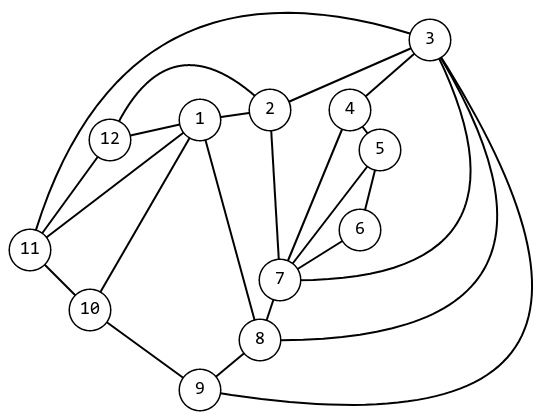
\includegraphics[height=6cm]{graph_1.png}
\end{center}
Удалим из $\psi_G$ рёбра, вошедшие в эти множества:\\
$\psi_{1} = \{\}$ \\
$\psi_{2} = \{\}$ \\
$\psi_{3} = \{\}$ \\
$\psi_{4} = \{u_{4 | 10}\}$ \\
$\psi_{5} = \{u_{4 | 10},u_{6 | 10}\}$ \\
$\psi_{6} = \{\}$ \\
$\psi_{7} = \{u_{4 | 12},u_{4 | 10}\}$ \\
$\psi_{8} = \{u_{4 | 12},u_{4 | 10},u_{6 | 10}\}$ \\
$\psi_{9} = \{u_{4 | 12},u_{5 | 12},u_{6 | 10}\}$ \\
$\psi_{10} = \{u_{4 | 12},u_{5 | 12},\}$ \\
$\psi_{11} = \{\}$ \\
$\psi_{12} = \{u_{4 | 10}\}$ \\
$\psi_{13} = \{u_{4 | 10},u_{6 | 10}\}$ \\
$\psi_{14} = \{\}$ \\
$\psi_{15} = \{u_{4 | 10}\}$ \\
$\psi_{16} = \{u_{4 | 10},u_{6 | 10}\}$ \\
Удалим пустые и объеденим одинаковые множества:\\
$\psi_{4} = \{u_{4 | 10}\}$ \\
$\psi_{5} = \{u_{4 | 10},u_{6 | 10}\}$ \\
$\psi_{7} = \{u_{4 | 12},u_{4 | 10}\}$ \\
$\psi_{8} = \{u_{4 | 12},u_{4 | 10},u_{6 | 10}\}$ \\
$\psi_{9} = \{u_{4 | 12},u_{5 | 12},u_{6 | 10}\}$ \\
$\psi_{10} = \{u_{4 | 12},u_{5 | 12},\}$ \\
Вычислим новые значения критерия:\\
$\alpha_{45} = |\psi_{4}| + |\psi_{5}| - |\psi_{4} \cap \psi_{5}| = 1+2-1=2$\\
$\alpha_{47} = |\psi_{4}| + |\psi_{7}| - |\psi_{4} \cap \psi_{7}| = 1+2-1=2$\\
$\alpha_{48} = |\psi_{4}| + |\psi_{8}| - |\psi_{4} \cap \psi_{8}| = 1+3-1=3$\\
$\alpha_{49} = |\psi_{4}| + |\psi_{9}| - |\psi_{4} \cap \psi_{9}| = 1+3=4$\\
$\alpha_{410} = |\psi_{4}| + |\psi_{10}| - |\psi_{4} \cap \psi_{10}| = 1+2-1=3$\\
$\alpha_{57} = |\psi_{5}| + |\psi_{7}| - |\psi_{5} \cap \psi_{7}| = 2+2-1=3$\\
$\alpha_{58} = |\psi_{5}| + |\psi_{8}| - |\psi_{5} \cap \psi_{8}| = 2+3-2=3$\\
$\alpha_{59} = |\psi_{5}| + |\psi_{9}| - |\psi_{5} \cap \psi_{9}| = 2+3-1=4$\\
$\alpha_{510} = |\psi_{5}| + |\psi_{10}| - |\psi_{5} \cap \psi_{10}| = 2+2=4$\\
$\alpha_{78} = |\psi_{7}| + |\psi_{8}| - |\psi_{7} \cap \psi_{8}| = 2+3-2=3$\\
$\alpha_{79} = |\psi_{7}| + |\psi_{9}| - |\psi_{7} \cap \psi_{9}| = 2+3-1=4$\\
$\alpha_{710} = |\psi_{7}| + |\psi_{10}| - |\psi_{7} \cap \psi_{10}| = 2+2-1=3$\\
$\alpha_{89} = |\psi_{8}| + |\psi_{9}| - |\psi_{8} \cap \psi_{9}| = 3+3-2=4$\\
$\alpha_{810} = |\psi_{8}| + |\psi_{10}| - |\psi_{8} \cap \psi_{10}| = 3+2-1=4$\\
$\alpha_{910} = |\psi_{9}| + |\psi_{10}| - |\psi_{9} \cap \psi_{10}| = 3+2-2=3$\\

\begin{tabular}{|c|c|c|c|c|c|c|c|c|c|c|c|c|c|c|c|c|}
    \hline
    & $\psi_{4}$ & $\psi_{5}$ & $\psi_{7}$ & $\psi_{8}$ & $\psi_{9}$ & $\psi_{10}$ \\
    \hline
    $\psi_{4}$  & 0 & 2  & 2 & 3  & 4  & 3  \\
    \hline
    $\psi_{5}$  &   & 0  & 3 & 3  & 4  & 4  \\
    \hline
    $\psi_{7}$  &   &    & 0 & 3  & 4  & 3  \\
    \hline
    $\psi_{8}$  &   &    &   & 0  & 4  & 4  \\
    \hline
    $\psi_{9}$  &   &    &   &    & 0  & 3  \\
    \hline
    $\psi_{10}$ &   &    &   &    &    & 0  \\
    \hline
\end{tabular}\\
\hfill\break
$\max \alpha_{i-j}=4$\\
Этому соответствует пара $\psi_4$ и $\psi_9$, проведём внутри гамильтонова цикла рёбра $\psi_9$, а снаружи рёбра $\psi_4$:\\
\begin{center}
    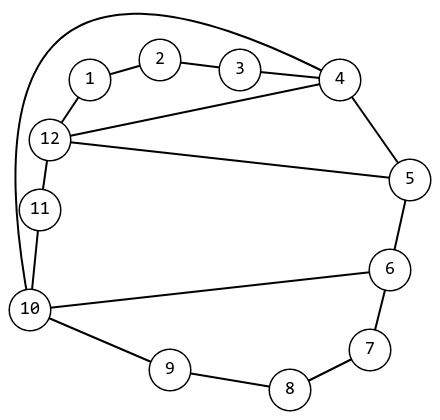
\includegraphics[height=6cm]{graph_2.png}
\end{center}
Удалим из $\psi_G$ рёбра, вошедшие в эти множества:\\
$\psi_{9} = \{\}$ \\
$\psi_{4} = \{\}$ \\
$\psi_{5} = \{\}$ \\
$\psi_{7} = \{\}$ \\
$\psi_{8} = \{\}$ \\
$\psi_{10} = \{\}$ \\
После удаления пустых множеств, $\psi_G=\{\}$, а значит граф планаризован\\
Толщина графа $m=2$
\end{document}